% ---------------------------------------------------------------------------
% Author guideline and sample document for EG publication using LaTeX2e input
% D.Fellner, v1.13, Jul 31, 2008

\documentclass{egpubl}
\usepackage{eg2017}

% --- for  Annual CONFERENCE
% \ConferenceSubmission   % uncomment for Conference submission
% \ConferencePaper        % uncomment for (final) Conference Paper
\STAR                   % uncomment for STAR contribution
% \Tutorial               % uncomment for Tutorial contribution
% \ShortPresentation      % uncomment for (final) Short Conference Presentation
% \Areas                  % uncomment for Areas contribution
% \MedicalPrize           % uncomment for Medical Prize contribution
% \Education              % uncomment for Education contribution
%
% --- for  CGF Journal
% \JournalSubmission    % uncomment for submission to Computer Graphics Forum
% \JournalPaper         % uncomment for final version of Journal Paper
%
% --- for  EG Workshop Proceedings
% \WsSubmission    % uncomment for submission to EG Workshop
% \WsPaper         % uncomment for final version of EG Workshop contribution
%
 \electronicVersion % can be used both for the printed and electronic version

% !! *please* don't change anything above
% !! unless you REALLY know what you are doing
% ------------------------------------------------------------------------

% for including postscript figures
% mind: package option 'draft' will replace PS figure by a filname within a frame
\ifpdf \usepackage[pdftex]{graphicx} \pdfcompresslevel=9
\else \usepackage[dvips]{graphicx} \fi

\PrintedOrElectronic

% prepare for electronic version of your document
\usepackage{t1enc,dfadobe}

\usepackage{egweblnk}
\usepackage{cite}

%%%%%%%%%%%%%%%%%%%%%%%%%%%%%%%%%%%%%%%%%%%%%%%%%%%%%%%%%%%%%%%%
\usepackage{graphicx}	% A package for graphics use (see figures)

%% subfigure and subcaption
\usepackage{caption}
\usepackage{subcaption}
%% bookmark
\usepackage{hyperref}
\usepackage{bookmark,hyperref}
%% url
\usepackage{url}

%% Math Packages %%%%%%%%%%%%%%%%%%%%%%%%%%%%%%%%%%%%%%%%%%%%
\usepackage{amssymb}
\usepackage{amsmath}
\usepackage{amsfonts}

% other packages
\usepackage{braket}

%for including pdf
\usepackage{pdfpages}
\graphicspath{{figures/}{images/}}
%%%%%%%%%%%%%%%%%%%%%%%%%%%%%%%%%%%%%%%%%%%%%%%%%%%%%%%%%%%%%%%%

% For backwards compatibility to old LaTeX type font selection.
% Uncomment if your document adheres to LaTeX2e recommendations.
% \let\rm=\rmfamily    \let\sf=\sffamily    \let\tt=\ttfamily
% \let\it=\itshape     \let\sl=\slshape     \let\sc=\scshape
% \let\bf=\bfseries

% end of prologue

% ---------------------------------------------------------------------
% EG author guidelines plus sample file for EG publication using LaTeX2e input
% D.Fellner, v1.17, Sep 23, 2010


\title%[EG \LaTeX\ Author Guidelines]%
{
%\LaTeX\ Author Guidelines for EUROGRAPHICS Proceedings Manuscripts
EG STARs
}

% for anonymous conference submission please enter your SUBMISSION ID
% instead of the author's name (and leave the affiliation blank) !!
\author%[D. Fellner \& S. Behnke]
{
%	D.\,W. Fellner\thanks{Chairman Eurographics Publications Board}$^{1,2}$
%	and S. Behnke$^{2}$
%	%        S. Spencer$^2$\thanks{Chairman Siggraph Publications Board}
%	\\
%	% For Computer Graphics Forum: Please use the abbreviation of your first name.
%	$^1$TU Darmstadt \& Fraunhofer IGD, Germany\\
%	$^2$Institut f{\"u}r ComputerGraphik \& Wissensvisualisierung, TU Graz, Austria
%	%        $^2$ Another Department to illustrate the use in papers from authors
%	%             with different affiliations
}

% ------------------------------------------------------------------------

% if the Editors-in-Chief have given you the data, you may uncomment
% the following five lines and insert it here
%
% \volume{27}   % the volume in which the issue will be published;
% \issue{1}     % the issue number of the publication
% \pStartPage{1}      % set starting page


%-------------------------------------------------------------------------
\begin{document}
	
%	\teaser{
%		
\includegraphics[width=\linewidth]{eg_new}
%		\centering
%		\caption{New EG Logo}
%		\label{fig:teaser}
%	}
	
\maketitle

\begin{abstract}
	The ABSTRACT is to be in fully-justified italicized text, 
	between two horizontal lines,
	in one-column format, 
	below the author and affiliation information. 
	Use the word ``Abstract'' as the title, in 9-point Times, boldface type, 
	left-aligned to the text, initially capitalized. 
	The abstract is to be in 9-point, single-spaced type.
	The abstract may be up to 3 inches (7.62 cm) long. \\
	Leave one blank line after the abstract, 
	then add the subject categories according to the ACM Classification Index 
	(see http://www.acm.org/class/1998/).
	
	\begin{classification} % according to http://www.acm.org/class/1998/
		\CCScat{Computer Graphics}{I.3.3}{Picture/Image Generation}{Line and curve generation}
	\end{classification}
	
\end{abstract}





%-------------------------------------------------------------------------
\section{Introduction}


%-------------------------------------------------------------------------	
\section{Visibility Histograms and Visibility-Driven Transfer Functions}
Visibility has been studied in measuring viewpoint quality \cite{bordoloi_view_2005} and enhancing ghost and cutaway views \cite{viola_importance-driven_2004} in volume visualization.
%\cite{bordoloi_view_2005}
%\cite{takahashi_feature-driven_2005}

In traditional transfer function design, the visibility of structures revealed in volume rendering is a consequence of adjusting transfer function parameters, rather than a design parameter \cite{preim_visual_2013}.
Correa and Ma \cite{correa_visibility-driven_2009} introduced visibility histograms to guide transfer function design for both manual and automatic adjustment.
Visibility histograms (Figure~\ref{fig:correa_visibility-driven_2009}), which summarize the distribution of visibility of voxels from a given viewpoint, are powerful feedback mechanisms of volume visualization \cite{emsenhuber_visibility_2008}.
Visibility histograms encode the information required to measure the efficacy of transfer functions and are advantageous in guiding and automating the manipulation of transfer functions.

\begin{figure}
	\centering
	\begin{minipage}{.24\textwidth}
		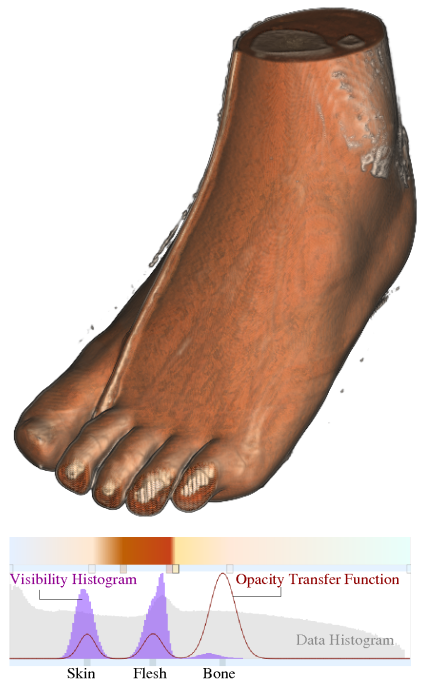
\includegraphics[width=1\linewidth]{images/correa_visibility-driven_2009_a}
		\subcaption{A user-defined opacity transfer function and the initial visibility histogram}
	\end{minipage}~
	\begin{minipage}{.24\textwidth}
		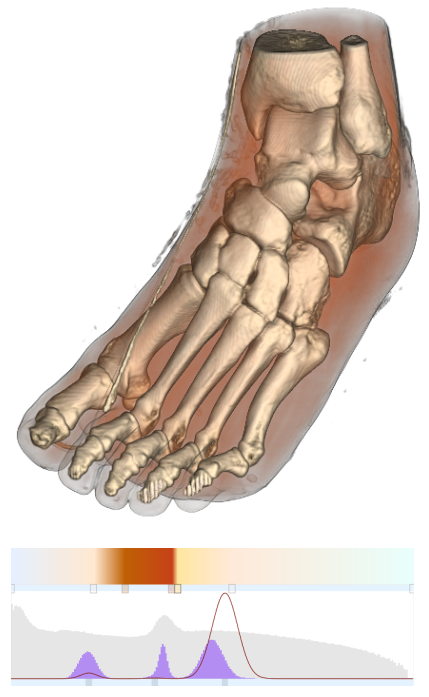
\includegraphics[width=1\linewidth]{images/correa_visibility-driven_2009_b}
		\subcaption{Here the visibility histogram has been modified to match the user-defined opacity transfer function.}
	\end{minipage}
	\caption{Visibility histograms \cite{correa_visibility-driven_2009}}
	\label{fig:correa_visibility-driven_2009}
\end{figure}

%Wang et al. \cite{wang_efficient_2011} extended visibility histograms to feature visibility, 
Wang et al. \cite{wang_efficient_2011} extended the previous work on visibility histograms and proposed a feature visibility metric,
in order to measure the influence of each feature to the volume rendered image. As shown in Figure~\ref{fig:wang_efficient_2011}, their approach allows the user to directly specify the desired visibility for the features of interest, and subsequently the opacity transfer function is optimized using an active set algorithm \cite{polyak_conjugate_1969}.

\begin{figure}
	\centering
	\begin{minipage}{.24\textwidth}
		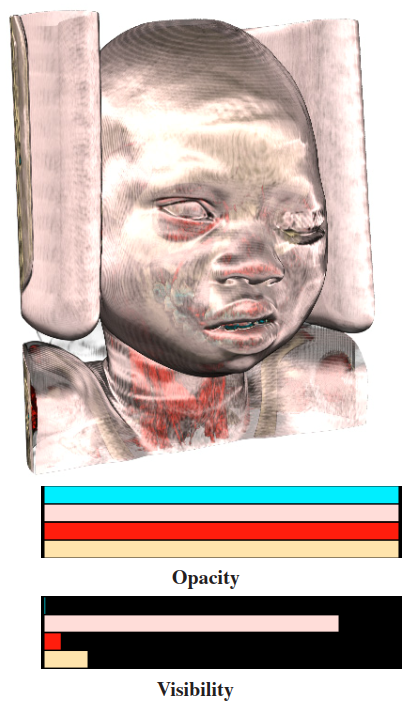
\includegraphics[width=1\linewidth]{images/wang_efficient_2011_a}
		\subcaption{Feature opacities are equal}
	\end{minipage}~
	\begin{minipage}{.24\textwidth}
		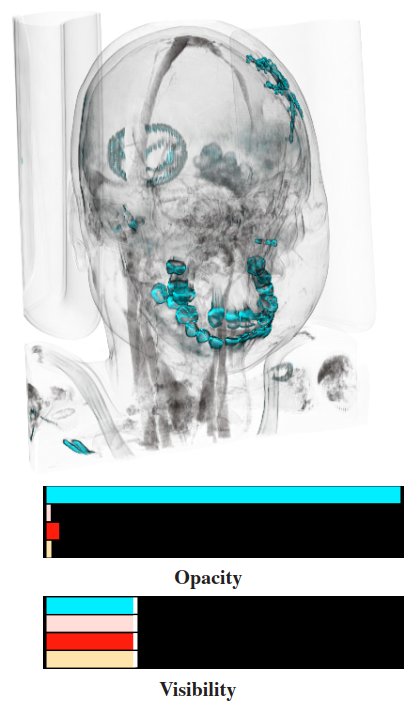
\includegraphics[width=1\linewidth]{images/wang_efficient_2011_b}
		\subcaption{Feature visibilities are equal}
	\end{minipage}
	\caption{Opacities and feature visibilities of 4 features highlighted in different colors \cite{wang_efficient_2011}}
	\label{fig:wang_efficient_2011}
\end{figure}

Ruiz et al. \cite{ruiz_automatic_2011} proposed an information-theoretic framework which obtains opacity transfer functions by minimizing the Kullback-Leibler divergence between the observed visibility distribution and a target distribution provided by the user. Later, Bramon et al. \cite{bramon_information_2013} extended this approach to visualize multimodal volume data.

Cai et al. \cite{cai_automatic_2013} described a method to derive opacity transfer functions by minimizing the Jensen-Shannon divergence between the observed visibility distribution and a user-defined target distribution. The target distribution can be defined using Gaussian function weighting.

%\cite{wan_fast_2010}
%%Fast volumetric data exploration with importance-based accumulated transparency modulation

%\cite{mak_visibility-aware_2011}
%%Visibility-Aware Direct Volume Rendering

%\cite{tang_depth-based_2011}
%%Depth-Based Feature Enhancement for Volume Visualization

%\cite{zhou_opacity_2014}
%%Opacity modulation based peeling for direct volume rendering

In addition, various methods were proposed regarding the use of visibility for enhancing different aspects of volume visualization.
Marchesin et al. \cite{marchesin_per-pixel_2010} introduced a volume rendering technique that manipulates the voxel opacity values in a view-dependent way, in order to enhance visibility of internal structures in the volume data set.
Bronstad et al. \cite{bronstad_visibility_2012} described local opacity transfer functions with feature detection along the ray profile implemented on the GPU. In their approach, visibility histograms are employed to access the performance of the feature detection algorithm.

Jung et al. \cite{jung_dual-modal_2012} presented a dual-modal visualization method, which uses visibility metrics to provide visual feedback regarding the occlusion caused by the volume data in one modal on the other modal.
Jung et al. \cite{jung_visibility-driven_2013} extended visibility histograms to multimodal volume visualization.
They demonstrated the use of visibility histograms together with region of interest segmentation was effective in visualizing PET-CT volume data sets.

Instead of computing the visibility of all voxels, Zheng et al. \cite{zheng_visibility_2013} employed local visibility histograms to ensure both the features of interest and contextual information are visible in multimodal volume visualization.
Schlegel and Pajarola \cite{schlegel_visibility-difference_2013} proposed a visibility-difference entropy metric. They presented an automated approach using this metric for generating a set of transfer function candidates with high ratings and are strongly distinct in what they reveal.

Qin et al. \cite{qin_voxel_2015} presented the voxel visibility model as a quality metric for transfer function design.
The voxel visibility model is a mapping function from data attributes of voxels to their visibility attributes. Instead of specifying transfer functions, this approach allows users to directly adjust the visibility of each voxel, and then the corresponding opacity transfer functions can be obtained by minimizing the distance between the desired voxel visibility distriubtion and the actual voxel visibility distribution.

%-------------------------------------------------------------------------
\subsection{Visibility-Based Sketching and Picking}

Sketching

The visibility of a sample refers to the alpha contribution of a sample to the final image, taking into account also the degree to which it is occluded by other samples in the view.
%This visibility can be computed as the difference between the accumulated alpha of a sample and the accumulated alpha of the previous sample along a ray in volume ray-casting.
%Correa et al. presented the general notion of visibility histograms \cite{correa_visibility_2011} which represent the distribution of visibility over intensity ranges in a volume rendering image.

Guo et al. \cite{guo_wysiwyg_2011} proposed a sketch-based manipulation technique for volume visualization based on clustering of depth, visibility, alpha and intensity. Subsequently, they described another sketch-based technique to specify local transfer functions for topology regions using contour trees \cite{guo_local_2013}. 

Picking

Wiebel et al. \cite{wiebel_wysiwyp:_2012} found that the user usually perceives features at a screen position with the highest visibility along the ray and they exploited this information in their volume picking technique.

Stoppel et al. \cite{elmqvist_visibility-driven_2014}

%-------------------------------------------------------------------------
	\subsection{Conclusions}

	
%-------------------------------------------------------------------------
	
%\bibliographystyle{eg-alpha}
\bibliographystyle{eg-alpha-doi-gv2}
	
\bibliography{bibliography}
	
%-------------------------------------------------------------------------
	
\end{document}

